\documentclass[12pt]{article}

% =============================================================================
% Paquetes y formato
% =============================================================================
\usepackage[utf8]{inputenc}
\usepackage[spanish,es-nodecimaldot]{babel}
\usepackage[margin=0.82in]{geometry}
\usepackage{amsmath,amsthm,amssymb,bm}
\usepackage{graphicx}
\usepackage{xcolor}

\definecolor{cideblue}{RGB}{5,35,75}
\definecolor{cidegray}{RGB}{80,85,92}

\graphicspath{{Figuras/Equilibrio_General/}}

\setlength{\parindent}{0pt}
\setlength{\parskip}{0.55em}
\allowdisplaybreaks
\pagestyle{plain}

\newtheoremstyle{cideplain}
  {0.8em}{0.8em}{\itshape}{}%
  {\bfseries\color{cideblue}}{.}{0.5em}{}
\newtheoremstyle{cidedef}
  {0.8em}{0.8em}{}{}%
  {\bfseries\color{cideblue}}{.}{0.5em}{}

\theoremstyle{cideplain}
\newtheorem{theorem}{Teorema}[section]
\newtheorem{proposition}[theorem]{Proposición}
\newtheorem{lemma}[theorem]{Lema}
\newtheorem{corollary}[theorem]{Corolario}

\theoremstyle{cidedef}
\newtheorem{definition}[theorem]{Definición}
\newtheorem{example}[theorem]{Ejemplo}
\newtheorem{remark}[theorem]{Observación}

\renewcommand{\proofname}{Demostración}
\DeclareMathOperator*{\argmax}{arg\,max}
\DeclareMathOperator{\MRS}{MRS}
\DeclareMathOperator{\MRT}{MRT}

\newcommand{\R}{\mathbb{R}}
\newcommand{\p}{\bm p}
\newcommand{\e}{\bm e}
\newcommand{\x}{\bm x}
\newcommand{\y}{\bm y}
\newcommand{\z}{\bm z}

% Referencias sin etiquetas cuadradas en la lista final.
\makeatletter
\renewenvironment{thebibliography}[1]
  {\section*{\refname}
   \list{}{\setlength{\leftmargin}{0pt}
           \setlength{\itemindent}{0pt}
           \setlength{\labelwidth}{0pt}
           \setlength{\labelsep}{0pt}
           \setlength{\itemsep}{0.7em}}
   \renewcommand\makelabel[1]{}
   \sloppy}
  {\endlist}
\makeatother

% =============================================================================
\begin{document}
% =============================================================================

\begin{center}
  {\large\bfseries Centro de Investigación y Docencia Económicas}\\[0.25em]
  {\large\bfseries Macroeconomía II --- Licenciatura en Economía}\\[0.8em]
  {\LARGE\bfseries\color{cideblue} Equilibrio general con dos bienes}\\[0.6em]
  {\large Consumidor y productor representativos; intercambio y producción}\\[0.8em]
  Arturo López Pérez \hfill Otoño de 2026
\end{center}

\vspace{0.5em}
\hrule
\vspace{1.0em}

% =============================================================================
\section{Dos bienes y agentes representativos}
% =============================================================================

\subsection{El consumidor representativo}

Considere dos bienes, \(1\) y \(2\), un vector de precios
\(\p=(p_1,p_2)\gg\bm 0\) y un consumidor representativo con preferencias
representadas por

\[
  u:\R_+^2\longrightarrow\R.
\]

Supondremos que \(u\) es continua, localmente no saciable y cuasicóncava. Dado un ingreso
monetario \(m>0\), el consumidor resuelve

\begin{equation}
  \x(\p,m)
  \in
  \argmax_{\x\in\R_+^2}
  \left\{u(\x):\p\cdot\x\leq m\right\}.
  \label{eq:rep-consumer}
\end{equation}

La solución \(\x(\p,m)=(x_1(\p,m),x_2(\p,m))\) es su demanda marshalliana.
Si la solución es única, cada componente es una función; si existen varias soluciones,
la demanda es una correspondencia.

En una solución interior y diferenciable,

\begin{equation}
  \MRS_{12}(\x)
  \equiv
  \frac{\partial u(\x)/\partial x_1}
       {\partial u(\x)/\partial x_2}
  =
  \frac{p_1}{p_2}.
  \label{eq:rep-consumer-foc}
\end{equation}

La tasa marginal de sustitución mide cuántas unidades del bien \(2\) valora el consumidor
como equivalentes a una unidad adicional del bien \(1\). El precio relativo \(p_1/p_2\)
mide el costo de esa sustitución en el mercado.

\begin{remark}[Interpretación del agente representativo]
Si existe una masa unitaria de consumidores idénticos, su demanda individual coincide con
la demanda agregada. Si la masa es distinta de uno, la demanda individual debe multiplicarse
por dicha masa. La representación no afirma que literalmente exista una sola persona.
\end{remark}

\subsection{El productor representativo}

Una empresa representativa dispone de un conjunto de producción
\(Y\subseteq\R^2\). Un vector \(\y=(y_1,y_2)\in Y\) describe producción
\emph{neta}: una componente positiva es un producto y una componente negativa es un insumo.
Como la empresa es precio-aceptante, resuelve

\begin{equation}
  \y(\p)
  \in
  \argmax_{\y\in Y}\p\cdot\y,
  \qquad
  \pi(\p)=\p\cdot\y(\p).
  \label{eq:rep-firm}
\end{equation}

Para interpretar la elección, suponga que la empresa transforma el bien \(1\) en el bien
\(2\). Si utiliza \(a\geq0\) unidades del bien \(1\) y produce \(F(a)\) unidades del bien
\(2\), entonces

\[
  \y(a)=(-a,F(a))
\]

y su problema es

\begin{equation}
  \max_{a\geq0}\left\{p_2F(a)-p_1a\right\}.
  \label{eq:transformation-firm}
\end{equation}

En una solución interior,

\begin{equation}
  F'(a^*)=\frac{p_1}{p_2}.
  \label{eq:firm-foc}
\end{equation}

El lado izquierdo es la tasa marginal de transformación: cuántas unidades adicionales del
bien \(2\) pueden producirse empleando una unidad adicional del bien \(1\). La empresa
iguala esa transformación tecnológica al precio relativo.

\subsection{Equilibrio parcial}

Para estudiar aisladamente el mercado del bien \(i\), se permite variar \(p_i\) y se
mantienen fijos \(p_{-i}\), el ingreso y los demás parámetros. Denote por
\(x_i^d(p_i;p_{-i},m)\) la demanda del consumidor y por
\(s_i(p_i;p_{-i})\) los recursos ofrecidos por la empresa y las dotaciones existentes.

\begin{definition}[Equilibrio parcial]
Un equilibrio parcial en el mercado del bien \(i\) es un precio \(p_i^*>0\) y una cantidad
\(q_i^*\) tales que

\begin{equation}
  x_i^d(p_i^*;p_{-i},m)
  =
  q_i^*
  =
  s_i(p_i^*;p_{-i}).
  \label{eq:partial-equilibrium}
\end{equation}
\end{definition}

En \(p_i^*\), la decisión óptima del consumidor coincide con la decisión óptima de la
empresa y el mercado se vacía. El calificativo \emph{parcial} es esencial: el análisis
excluye la retroalimentación de este mercado sobre \(p_{-i}\), el ingreso y el resto de
la economía.

% =============================================================================
\section{Intercambio puro: asignaciones antes de introducir precios}
% =============================================================================

\subsection{Dos bienes y dos agentes}

Considere dos agentes, \(A\) y \(B\), y dos bienes. No existe producción: todos los
recursos provienen de las dotaciones iniciales

\[
  \e^A=(e_1^A,e_2^A),
  \qquad
  \e^B=(e_1^B,e_2^B).
\]

La dotación agregada es

\[
  \overline{\e}
  =
  \e^A+\e^B
  =
  (\overline e_1,\overline e_2)\gg\bm 0.
\]

Una asignación es un par \((\x^A,\x^B)\). Es factible si

\begin{equation}
  \x^A+\x^B\leq\overline{\e}.
  \label{eq:exchange-feasibility}
\end{equation}

Con preferencias localmente no saciables, toda asignación eficiente utiliza completamente
los recursos y \eqref{eq:exchange-feasibility} se cumple con igualdad.

\begin{figure}[htbp]
  \centering
  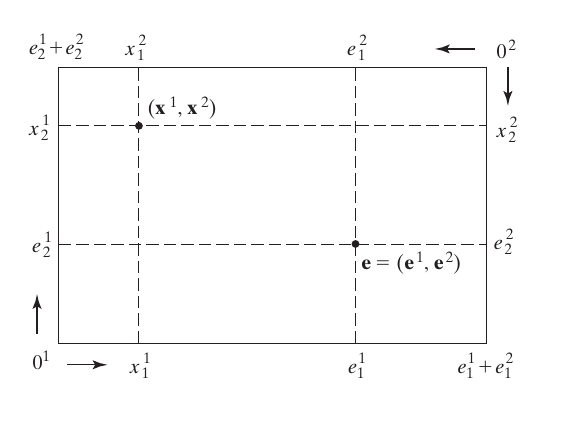
\includegraphics[width=0.72\textwidth]{edgeworth_caja.png}
  \caption{Caja de Edgeworth para dos bienes y dos agentes. Las cantidades del agente
  \(A\) se miden desde el origen suroeste y las de \(B\) desde el origen noreste. Los
  agentes 1 y 2 de la figura corresponden a \(A\) y \(B\), respectivamente.
  Fuente: (Jehle y Reny, 2011, fig. 5.1).}
  \label{fig:edgeworth-basic-two}
\end{figure}
\clearpage

La caja tiene ancho \(\overline e_1\) y altura \(\overline e_2\). Una vez elegida
\(\x^A\), la canasta de \(B\) queda determinada por factibilidad:

\[
  \x^B=\overline{\e}-\x^A.
\]

\subsection{Eficiencia de Pareto}

\begin{definition}[Mejora de Pareto]
Una asignación factible \((\widehat{\x}^A,\widehat{\x}^B)\) es una mejora de Pareto
respecto de \((\x^A,\x^B)\) si

\[
  u^h(\widehat{\x}^h)\geq u^h(\x^h),
  \qquad h\in\{A,B\},
\]

y al menos una de las dos desigualdades es estricta.
\end{definition}

\begin{definition}[Eficiencia de Pareto]
Una asignación factible es eficiente en el sentido de Pareto si no existe otra asignación
factible que constituya una mejora de Pareto.
\end{definition}

Si las preferencias son diferenciables, estrictamente crecientes y estrictamente
cuasicóncavas, toda asignación interior eficiente satisface

\begin{equation}
  \MRS_{12}^A(\x^A)
  =
  \MRS_{12}^B(\x^B).
  \label{eq:mrs-equality}
\end{equation}

Si las tasas marginales de sustitución fueran diferentes, existiría una tasa de intercambio
intermedia que permitiría mejorar a ambos agentes. Por tanto, la igualdad en
\eqref{eq:mrs-equality} elimina las ganancias marginales de intercambio aún no explotadas.

Las asignaciones eficientes también pueden obtenerse, para cada peso social
\(\lambda\in(0,1)\), mediante

\begin{equation}
  \max_{\x^A,\x^B}
  \lambda u^A(\x^A)+(1-\lambda)u^B(\x^B)
  \quad\text{sujeto a}\quad
  \x^A+\x^B=\overline{\e}.
  \label{eq:planner-exchange-two}
\end{equation}

Variar \(\lambda\) recorre la curva de contrato. En esta sección todavía no existen precios:
únicamente se han descrito factibilidad y eficiencia, es decir, el lado real de la economía.

\begin{figure}[htbp]
  \centering
  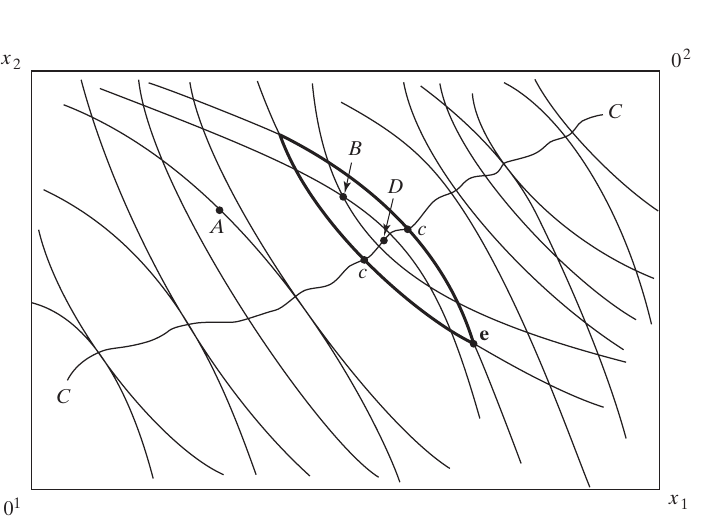
\includegraphics[width=0.78\textwidth]{edgeworth_contrato.png}
  \caption{Curvas de indiferencia y curva de contrato \(C\). Los agentes 1 y 2 de la
  figura corresponden a \(A\) y \(B\). Fuente: (Jehle y Reny, 2011, fig. 5.2).}
  \label{fig:edgeworth-contract-two}
\end{figure}
\clearpage

% =============================================================================
\section{Economía de mercado: precios y equilibrio walrasiano}
% =============================================================================

\subsection{Decisiones descentralizadas}

Introduzca un vector de precios \(\p=(p_1,p_2)\gg\bm 0\). En intercambio puro,
el ingreso de cada agente es el valor de su dotación:

\[
  m^h(\p)=\p\cdot\e^h,
  \qquad h\in\{A,B\}.
\]

Cada agente toma los precios como dados y resuelve

\begin{equation}
  \x^h(\p)
  \in
  \argmax_{\x^h\geq\bm 0}
  \left\{
    u^h(\x^h):
    \p\cdot\x^h\leq\p\cdot\e^h
  \right\}.
  \label{eq:consumer-market-two}
\end{equation}

\begin{definition}[Equilibrio walrasiano]
Un equilibrio walrasiano es un vector de precios \(\p^*\gg\bm 0\) y una asignación
\((\x^{A*},\x^{B*})\) tales que:

\begin{enumerate}
  \item para cada \(h\in\{A,B\}\), \(\x^{h*}\) resuelve
  \eqref{eq:consumer-market-two} a precios \(\p^*\);
  \item ambos mercados se vacían:
  \begin{equation}
    \x^{A*}+\x^{B*}=\overline{\e}.
    \label{eq:market-clearing-two}
  \end{equation}
\end{enumerate}
\end{definition}

Defina la demanda excedente agregada:

\begin{equation}
  \z(\p)
  =
  \x^A(\p)+\x^B(\p)-\overline{\e}.
  \label{eq:excess-demand-two}
\end{equation}

Su componente \(z_i(\p)\) es positiva si existe exceso de demanda del bien \(i\) y negativa
si existe exceso de oferta. Los precios de equilibrio satisfacen

\[
  \z(\p^*)=\bm 0.
\]

\begin{proposition}[Ley de Walras]
Si las preferencias son localmente no saciables, entonces

\[
  \p\cdot\z(\p)=0
\]

para todo \(\p\gg\bm 0\).
\end{proposition}

\begin{proof}
La no saciedad local implica que cada restricción presupuestaria se cumple con igualdad:
\(\p\cdot\x^h(\p)=\p\cdot\e^h\). Sumando sobre \(h=A,B\),

\[
  \p\cdot
  \left[
    \x^A(\p)+\x^B(\p)-\e^A-\e^B
  \right]
  =0,
\]

que es precisamente la ley de Walras.
\end{proof}

En una economía de dos bienes,

\[
  p_1z_1(\p)+p_2z_2(\p)=0.
\]

Por tanto, si un mercado se vacía, el otro también. Además, si las demandas son homogéneas
de grado cero en precios, sólo importa el precio relativo. Podemos normalizar \(p_2=1\) y
denotar

\[
  q\equiv\frac{p_1}{p_2}=p_1.
\]

\subsection{Un equilibrio Cobb--Douglas}

Suponga

\[
  u^A(\x^A)=(x_1^Ax_2^A)^{1/2},
  \qquad
  u^B(\x^B)=(x_1^Bx_2^B)^{1/2},
\]

y dotaciones especializadas

\[
  \e^A=(1,0),
  \qquad
  \e^B=(0,1).
\]

Al normalizar \(p_2=1\), los ingresos son

\[
  m^A(q)=q,
  \qquad
  m^B(q)=1.
\]

Las demandas marshallianas son

\begin{align}
  x_1^A(q)&=\frac12,
  &x_2^A(q)&=\frac q2,
  \label{eq:demands-a-two}\\
  x_1^B(q)&=\frac{1}{2q},
  &x_2^B(q)&=\frac12.
  \label{eq:demands-b-two}
\end{align}

Como la dotación agregada es \(\overline{\e}=(1,1)\), las demandas excedentes son

\begin{align}
  z_1(q)
  &=
  \frac12+\frac{1}{2q}-1
  =
  \frac{1-q}{2q},
  \label{eq:z1-two}\\
  z_2(q)
  &=
  \frac q2+\frac12-1
  =
  \frac{q-1}{2}.
  \label{eq:z2-two}
\end{align}

Ambas se anulan únicamente cuando

\begin{equation}
  q^*=\frac{p_1^*}{p_2^*}=1.
  \label{eq:qstar-two}
\end{equation}

En equilibrio,

\[
  \x^{A*}=\x^{B*}
  =
  \left(\frac12,\frac12\right).
\]

El agente \(A\) entrega media unidad del bien \(1\) a cambio de media unidad del bien \(2\),
mientras que \(B\) realiza el intercambio opuesto.

\subsection{Un precio relativo que no es de equilibrio}

Considere ahora el precio relativo

\[
  q=\frac{p_1}{p_2}=2.
\]

El bien \(1\) es relativamente caro: una unidad cuesta dos unidades del bien \(2\).
Al evaluar \eqref{eq:demands-a-two}--\eqref{eq:demands-b-two}, se obtiene

\[
  X_1^D(2)
  =
  \frac12+\frac14
  =
  \frac34,
  \qquad
  X_2^D(2)
  =
  1+\frac12
  =
  \frac32.
\]

La comparación con la oferta disponible \(\overline{\e}=(1,1)\) es

\begin{center}
\small
\begin{tabular}{p{0.25\textwidth}p{0.19\textwidth}p{0.18\textwidth}p{0.25\textwidth}}
\hline
Mercado & Demanda agregada & Oferta disponible & Desequilibrio\\
\hline
Bien \(1\), relativamente caro
  & \(3/4\) & \(1\) & exceso de oferta de \(1/4\)\\
Bien \(2\), relativamente barato
  & \(3/2\) & \(1\) & exceso de demanda de \(1/2\)\\
\hline
\end{tabular}
\end{center}

Equivalentemente,

\[
  z_1(2)=-\frac14<0,
  \qquad
  z_2(2)=\frac12>0.
\]

Por tanto, \(q=2\) no es un precio relativo de equilibrio walrasiano. El bien cuyo precio
relativo es demasiado alto presenta exceso de oferta; el bien relativamente barato presenta
exceso de demanda. No obstante, la ley de Walras continúa cumpliéndose:

\[
  qz_1(q)+z_2(q)
  =
  2\left(-\frac14\right)+\frac12
  =
  0.
\]

\begin{proposition}[Signo del desequilibrio]
En este ejemplo:

\[
  q>1
  \quad\Longrightarrow\quad
  z_1(q)<0<z_2(q),
\]

mientras que

\[
  q<1
  \quad\Longrightarrow\quad
  z_2(q)<0<z_1(q).
\]

El mercado presiona a la baja el precio relativo del bien con exceso de oferta y al alza el
precio relativo del bien con exceso de demanda.
\end{proposition}

\begin{remark}[Precios relativos, no nivel de precios]
Multiplicar ambos precios por el mismo número no modifica presupuestos ni demandas reales.
Los vectores \((1,1)\) y \((5,5)\) representan el mismo precio relativo de equilibrio.
En cambio, \((2,1)\) representa \(q=2\) y no es proporcional al vector de equilibrio.
\end{remark}

\begin{figure}[htbp]
  \centering
  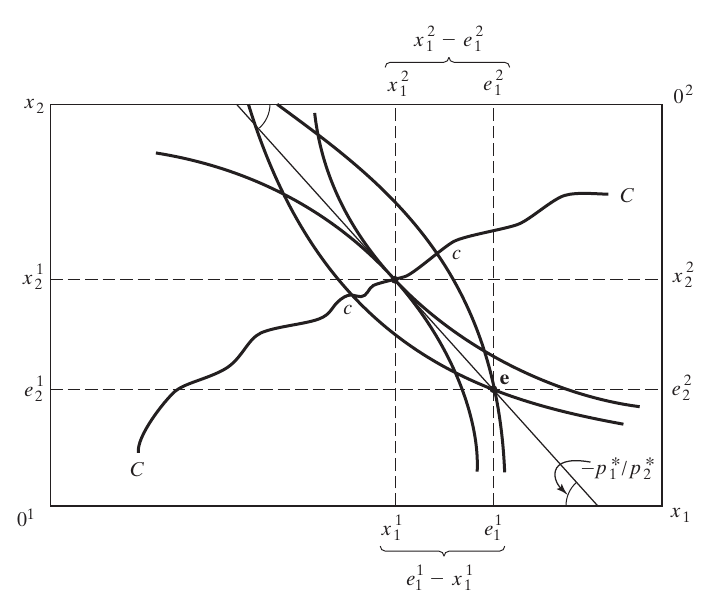
\includegraphics[width=0.78\textwidth]{edgeworth_walras.png}
  \caption{Equilibrio walrasiano en la caja de Edgeworth. La recta presupuestaria
  común pasa por la dotación inicial y, al precio relativo de equilibrio, las demandas
  de ambos agentes son compatibles. Fuente: elaboración basada en Jehle y Reny
  (2011, fig. 5.4).}
\end{figure}

\clearpage

% =============================================================================
\section{Bienestar y equilibrio competitivo}
% =============================================================================

El equilibrio walrasiano no sólo coordina decisiones individuales. Bajo condiciones
regulares, también selecciona una asignación eficiente.

\begin{theorem}[Primer teorema fundamental del bienestar]
Suponga que las preferencias de ambos consumidores son localmente no saciadas. Si
\((\p^*,\x^{A*},\x^{B*})\) es un equilibrio walrasiano, entonces la asignación
\((\x^{A*},\x^{B*})\) es eficiente en el sentido de Pareto.
\end{theorem}

\begin{proof}
Suponga, por contradicción, que existe una asignación factible
\((\widehat{\x}^{A},\widehat{\x}^{B})\) que constituye una mejora de Pareto. La
optimalidad de cada consumidor y la no saciedad local implican

\[
  \p^*\cdot\widehat{\x}^{h}
  \geq
  \p^*\cdot\e^{h},
  \qquad h\in\{A,B\},
\]

y la desigualdad es estricta para al menos uno de los dos agentes, pues alguno debe estar
estrictamente mejor. Al sumar,

\[
  \p^*\cdot
  \bigl(\widehat{\x}^{A}+\widehat{\x}^{B}\bigr)
  >
  \p^*\cdot(\e^{A}+\e^{B}).
\]

Esto contradice la factibilidad de la asignación alternativa. Por tanto, no existe una
mejora de Pareto.
\end{proof}

Cuando la solución es interior y las preferencias son diferenciables, el resultado puede
verse en términos de pendientes:

\[
  \MRS^{A}_{12}(\x^{A*})
  =
  \frac{p_1^*}{p_2^*}
  =
  \MRS^{B}_{12}(\x^{B*}).
\]

El precio relativo común alinea las tasas marginales de sustitución de ambos consumidores.
Esta igualdad es una condición necesaria de eficiencia interior, aunque por sí sola no
garantiza optimalidad global sin supuestos adicionales sobre las preferencias.

% =============================================================================
\section{Economía de mercado con producción}
% =============================================================================

Ahora se permite transformar recursos mediante una empresa representativa. Se mantienen
dos consumidores, \(A\) y \(B\), dos bienes y dotaciones iniciales
\(\e^{A},\e^{B}\in\R_+^2\). La empresa elige un plan de producción
\(\y=(y_1,y_2)\in Y\subset\R^2\), donde un componente negativo es un insumo neto y uno
positivo es un producto neto.

Los consumidores poseen participaciones \(\theta_A,\theta_B\geq 0\) en la empresa, con

\[
  \theta_A+\theta_B=1.
\]

De este modo, los beneficios no desaparecen: forman parte del ingreso de sus propietarios.

\subsection{La empresa y los consumidores}

A precios \(\p\gg\bm 0\), la empresa representativa resuelve

\[
  \y(\p)\in\argmax_{\y\in Y}\;\p\cdot\y,
  \qquad
  \pi(\p)=\p\cdot\y(\p).
\]

El ingreso del consumidor \(h\in\{A,B\}\) es el valor de su dotación más su participación
en los beneficios:

\[
  m^h(\p)
  =
  \p\cdot\e^h+\theta_h\pi(\p).
\]

Por tanto, su problema es

\[
  \x^h(\p)
  \in
  \argmax_{\x^h\in\R_+^2}
  \left\{
    u^h(\x^h):
    \p\cdot\x^h
    \leq
    \p\cdot\e^h+\theta_h\pi(\p)
  \right\}.
\]

\begin{definition}[Equilibrio walrasiano con producción]
Un equilibrio walrasiano con producción es un vector de precios
\(\p^*\gg\bm 0\), una asignación de consumo
\((\x^{A*},\x^{B*})\) y un plan \(\y^*\in Y\) tales que:

\begin{enumerate}
  \item cada consumidor maximiza su utilidad sujeto a su restricción presupuestaria;
  \item la empresa maximiza beneficios, es decir,
  \(\y^*\in\argmax_{\y\in Y}\p^*\cdot\y\);
  \item ambos mercados se vacían:
  \[
    \x^{A*}+\x^{B*}
    =
    \e^A+\e^B+\y^*.
  \]
\end{enumerate}
\end{definition}

La última igualdad representa dos condiciones simultáneas:

\[
  x_1^{A*}+x_1^{B*}=e_1^A+e_1^B+y_1^*,
  \qquad
  x_2^{A*}+x_2^{B*}=e_2^A+e_2^B+y_2^*.
\]

La producción amplía o transforma los recursos disponibles, pero no elimina la restricción
de factibilidad: el consumo agregado no puede exceder las dotaciones iniciales más la
producción neta.

\subsection{Eficiencia con producción}

\begin{definition}[Eficiencia de Pareto con producción]
Una asignación \((\x^A,\x^B,\y)\) es eficiente si es factible y no existe otra asignación
factible \((\widehat{\x}^A,\widehat{\x}^B,\widehat{\y})\) que mejore débilmente a ambos
consumidores y estrictamente a por lo menos uno.
\end{definition}

\begin{theorem}[Primer teorema del bienestar con producción]
Si las preferencias son localmente no saciadas, toda asignación de equilibrio walrasiano
con producción es eficiente en el sentido de Pareto.
\end{theorem}

\begin{proof}
Suponga que una asignación factible alternativa mejora en el sentido de Pareto al
equilibrio. La optimalidad de los consumidores implica

\[
  \sum_{h=A,B}\p^*\cdot\widehat{\x}^{h}
  >
  \sum_{h=A,B}
  \left(\p^*\cdot\e^h+\theta_h\pi^*\right)
  =
  \p^*\cdot(\e^A+\e^B)+\pi^*,
\]

donde se utilizó \(\theta_A+\theta_B=1\). Por maximización de beneficios,

\[
  \pi^*=\p^*\cdot\y^*
  \geq
  \p^*\cdot\widehat{\y}.
\]

Sin embargo, la factibilidad de la alternativa exige

\[
  \widehat{\x}^{A}+\widehat{\x}^{B}
  \leq
  \e^A+\e^B+\widehat{\y},
\]

componente a componente. Como \(\p^*\gg\bm 0\), esto contradice la primera desigualdad.
\end{proof}

\subsection{Interpretación con una tecnología de transformación}

Considere nuevamente una tecnología de la forma

\[
  \y(a)=(-a,F(a)),
  \qquad a\geq 0,
\]

donde la empresa utiliza \(a\) unidades del bien \(1\) para producir \(F(a)\) unidades del
bien \(2\). Su problema es

\[
  \max_{a\geq 0}\;p_2F(a)-p_1a.
\]

En una solución interior,

\[
  F'(a^*)=\frac{p_1^*}{p_2^*}.
\]

Si las elecciones de consumo también son interiores, el equilibrio satisface

\[
  \MRS_{12}^{A}(\x^{A*})
  =
  \MRS_{12}^{B}(\x^{B*})
  =
  \frac{p_1^*}{p_2^*}
  =
  \MRT_{12}(\y^*).
\]

Así, un único precio relativo coordina tres márgenes: la sustitución del consumidor \(A\),
la sustitución del consumidor \(B\) y la transformación tecnológica de la empresa.

\begin{remark}[Conexión con el modelo macroeconómico de un periodo]
El modelo de consumidor y empresa representativos del capítulo 5 de Williamson (2018)
es una versión agregada de esta estructura. El hogar elige consumo y ocio, la empresa
demanda trabajo y produce, y los precios ajustan hasta hacer compatibles todas las
decisiones. En ese caso, los dos mercados relevantes pueden expresarse como el mercado del
bien y el mercado de trabajo.
\end{remark}

% =============================================================================
\section{Síntesis}
% =============================================================================

\begin{center}
\small
\begin{tabular}{p{0.22\textwidth}p{0.31\textwidth}p{0.36\textwidth}}
\hline
Entorno & Decisiones & Condición central\\
\hline
Equilibrio parcial con agentes representativos
& El consumidor demanda y la empresa ofrece un bien; las demás variables se mantienen
fijas.
& La oferta y la demanda del mercado estudiado son iguales.\\[0.4em]
Intercambio puro sin precios
& Dos consumidores comparan asignaciones factibles.
& La eficiencia interior requiere igualdad de tasas marginales de sustitución.\\[0.4em]
Mercado de intercambio puro
& Cada consumidor maximiza sujeto al valor de su dotación.
& Un precio relativo hace que ambos mercados se vacíen.\\[0.4em]
Mercado con producción
& Los consumidores maximizan utilidad y la empresa maximiza beneficios.
& El consumo agregado es igual a las dotaciones más la producción neta.\\
\hline
\end{tabular}
\end{center}

\begin{remark}[Idea central]
El equilibrio general no consiste en encontrar por separado el cruce de oferta y demanda
de cada bien. Consiste en encontrar un mismo vector de precios relativos que haga
mutuamente compatibles todas las decisiones óptimas de consumo y producción.
\end{remark}

% =============================================================================
\section{Ejercicios}
% =============================================================================

\begin{enumerate}
  \item En el ejemplo Cobb--Douglas, calcule \(z_1(q)\) y \(z_2(q)\) para
  \(q=1/2\). Identifique el bien con exceso de oferta y el bien con exceso de demanda.

  \item Verifique directamente que \(qz_1(q)+z_2(q)=0\) para todo \(q>0\).
  Explique por qué no es posible que ambos mercados tengan exceso de demanda.

  \item Suponga ahora
  \(u^A(x_1^A,x_2^A)=(x_1^A)^{1/3}(x_2^A)^{2/3}\) y
  \(u^B(x_1^B,x_2^B)=(x_1^B)^{2/3}(x_2^B)^{1/3}\), manteniendo las dotaciones del
  ejemplo. Encuentre el precio relativo de equilibrio.

  \item En la economía con producción, demuestre que la suma de los ingresos de los
  consumidores es igual al valor de las dotaciones agregadas más los beneficios de la
  empresa.

  \item Explique por qué la igualdad
  \(\MRS_{12}^A=\MRS_{12}^B=\MRT_{12}\) resume la eficiencia en consumo y en producción
  cuando la solución es interior.
\end{enumerate}

\nocite{JehleReny2011,Williamson2018}
\bibliographystyle{apalike-es}
\bibliography{../Slides/References.bib.bib}

\end{document}
